\input{../../preambule.tex} 
\include{}
% Modification des variable de session 
\input{../../variables.tex} 

\newcommand{\exercice}{1}

% custom footers and headers
\usepackage{fancyhdr}
\pagestyle{fancy}
\lhead{\nomcours}
\chead{}
\rhead{\cours}
\lfoot{ Exercice \exercice}
\cfoot{}
\rfoot{Page \thepage}
\renewcommand{\headrulewidth}{1pt}
\renewcommand{\footrulewidth}{1pt}
%
% my own titles

\makeatletter
\renewcommand{\maketitle}{
	\begin{center}
		\vspace{2ex}
		{\huge \textsc{\@title}}
		\vspace{1ex}
		\\
		\linia\\
		\@author \hfill \@date
		
		\linia\\
		\vspace{2ex}
	\end{center}
}



\makeatother
%%%
%%%----------%%%----------%%%----------%%%----------%%%

\begin{document}
	
	\title{Exercice \textnumero{}\exercice \\
		\\Installation d'un client \\
		\SELinux
		
	}
	\author{\prof, \Cegep}
	\date{\session}
	
	
	  \maketitle
	
	\begin{flushleft}
		\noindent \textbf{Évaluation :} formative \\
		\textbf {Travail de préférence individuel.}\\
		\textbf{Durée :} 2 heures \\
		\textbf{Système d'exploitation :} \SELinux \\
		\textbf{Environnement de virtualisation :} \Esx\\
		\textbf{Couleur du texte :} En {\color{blue}bleu} :porté attention. 
		En {\color{orange}orange} des noms à modifier en fonction du contexte.

		
	\end{flushleft}
	\rule{17cm}{0.1pt}
	
	\section{Préparation de la machine virtuelle }
	
	vSphere nous permet d'utiliser trois méthodes pour avec accès à des machines virtuelles:
	\begin{enumerate}
		\item Création de la VM depuis un modèle. 
		\item Importer une VM depuis VM Workstation.
		\item \textbf{Création de la VM depuis un fichier iso, donc à partir de rien.}
	\end{enumerate}
	Nous allons utiliser cette dernière méthode.
	\subsection {Création de la VM depuis un fichier iso}
	
	
	\begin{itemize}
		\item  Sélectionnez le dossier {\color{blue}\DossierVM }  et créer votre sous-dossier dans le format :\\
		 ({\color{orange}\sousDossierVM}). 
		 \item En étant situé dans votre nouveau dossier, dans le menu Actions, sélectionnez {\color{blue}Nouvelle machine virtuelle}. 
				
		\item Dans la nouvelle fenêtre, {\color{blue}Créer une machine virtuelle} devrait être sélectionné par défaut. Alors, cliquez sur le bouton \textbf{NEXT}.
		
		\item Inscrivez le Nom de la machine de la façon suivante : {\color{orange}\nomVM}
		
		Cliquez sur le bouton \textbf{NEXT}.
		
		\item À l'étape 3, Contrôles de compatibilité effectués avec succès, cliquez sur le bouton \textbf{NEXT}.
		
		\item Sélectionner un stockage {\color{blue}SAN-DFC}. Cliquez sur le bouton \textbf{NEXT}.
			
		\item Sélectionnez une compatibilité, laissez la valeur par défaut et cliquez sur le bouton \textbf{NEXT}. 
	
		
		\item Sélectionner un système d'exploitation invité, Changer {\color{blue} Windows pour Linux} et dans Version du SE invité sélectionnez {\color{blue}Ubuntu Linux (64 bits) }.
		
		
		\item À la fenêtre {\color{blue}personnaliser le matériel} plusieurs modifications sont nécessaires : 
		\begin{itemize}
			\item \textbf{CPU} : 2
			\item \textbf{Memoire}: 4 Go
			\item \textbf{Nouveau disque dur} 40 Go
			\item \textbf{Nouveau lecteur CD/DVD} : Fichier ISO banque de données
			Vous devez sélectionner un fichier dans \(\Rightarrow\)  SAN-DFC \(\Rightarrow\)  ISO \(\Rightarrow\) \textbf{Ubuntu-20.04-desktop-amd64.iso}. Cliquez sur \textbf{OK}.
			\item \textbf{Attention : } N'oubliez pas de cochez connecter pour que le fichier ISO puise démarrer lors du premier démarrage de votre machine virtuelle.
			\item \textbf{Carte vidéo :} 256 Mo de Mémoire vidéo total et activer support 3D.
		\end{itemize}
		
		
		\item Finalement, vous êtes {\color{blue}prêt à terminer}. Vous avez un résumé de vos choix. Vérifiez le et cliquez sur \textbf{FINISH} si ça représente vos choix.
		\item Vous avez maintenant une nouvelle machine virtuelle placée dans votre sous-dossier. Elle ne demande qu'à être installée. {\color{orange}{\Huge \smiley{}}}
	\end{itemize}
	
	
	
	
	
	
	
	
	
	
	
	
	
	
	\section{Installation d'Ubuntu 20.04} 
	Lors du démarrage, le BIOS (par défaut) ou l'EFI de votre machine va vérifier la présence d'un CD/DVD, pareille comme un poste non virtualisé, si vous avez cocher connecter pour votre CD/DVD  Alors, nous pouvons procéder à l'installation depuis le fichier ISO d'Ubuntu 20.04.
	
	\begin{itemize}
		\item  Sélectionnez votre VM dans votre sous-dossier.
		\item Cliquez sur \textbf{Action} \(\Rightarrow\) Alimentation \(\Rightarrow\) Mettre sous tension.\\
		
		\vspace{1pt}
		
		\fcolorbox{black}{orange}{
			\begin{minipage}{15cm}
				Un avertissement vous informe que \textit{VMWare Tools n'est pas installé sur cette machine virtuelle}. Nous y reviendrons à la fin de l'installation. 
		\end{minipage}}
		
		\vspace{10pt}  
		
		\item Cliquez sur Lancer la console Web et à nouveau sur Console Web et OK.
		\item Si tous ces déroulés comme prévu, vous avez la page d'installation d'Ubuntu avec le choix de la langue.  Choisissez {\color{blue}Français} et {\color{blue}Install Ubuntu}.
		\item Disposition du Clavier. À cette étape, vous devez habituellement choisir le clavier utilisé dans votre organisation. Il ne s'agit pas d'un choix personnel. Sauf s'il s'agit de votre poste de travail personnel. Ce qui n'est pas le cas ici. 
		Donc sélectionnez {\color{blue}French(Canada)} et {\color{blue}French(Canada)- Canadien Multilingual} qui est habituellement le clavier utiliser au Québec.\\
		Vous pouvez tester votre clavier dans le champ texte réservé à cette fin.
		\item Cliquez sur \textbf{Continuer}.
		\item {\color{blue}Mises à jour et autres logiciels}, garder les options par défauts: {\color{blue}Installation normale} et {\color{blue}télécharger les mises à jour pendant l'installation d'Ubuntu}
		\item Cliquez sur \textbf{Continuer}.
		\item {\color{blue}Type d'installation} Ici nous allons opter pour {\color{blue} Autres chose} et cliquez sur \textbf{Continuer}.
	\end{itemize}
	\subsection{Préparation de l'espace disque}
	\begin{itemize}
		\item  Vous avez la fenêtre représentant le disque /dev/sda. Nous devons créer des partitions sur le disque pour avoir un système d'exploitation bien installé avec des partitions séparées pour le SE, pour les données variables et pour les usagers. Figure~\ref{Fig8}
		
		\begin{figure}[!htb]
			\centering
			\caption{\label{Fig8}Partition du disque dur /dev/sda}
			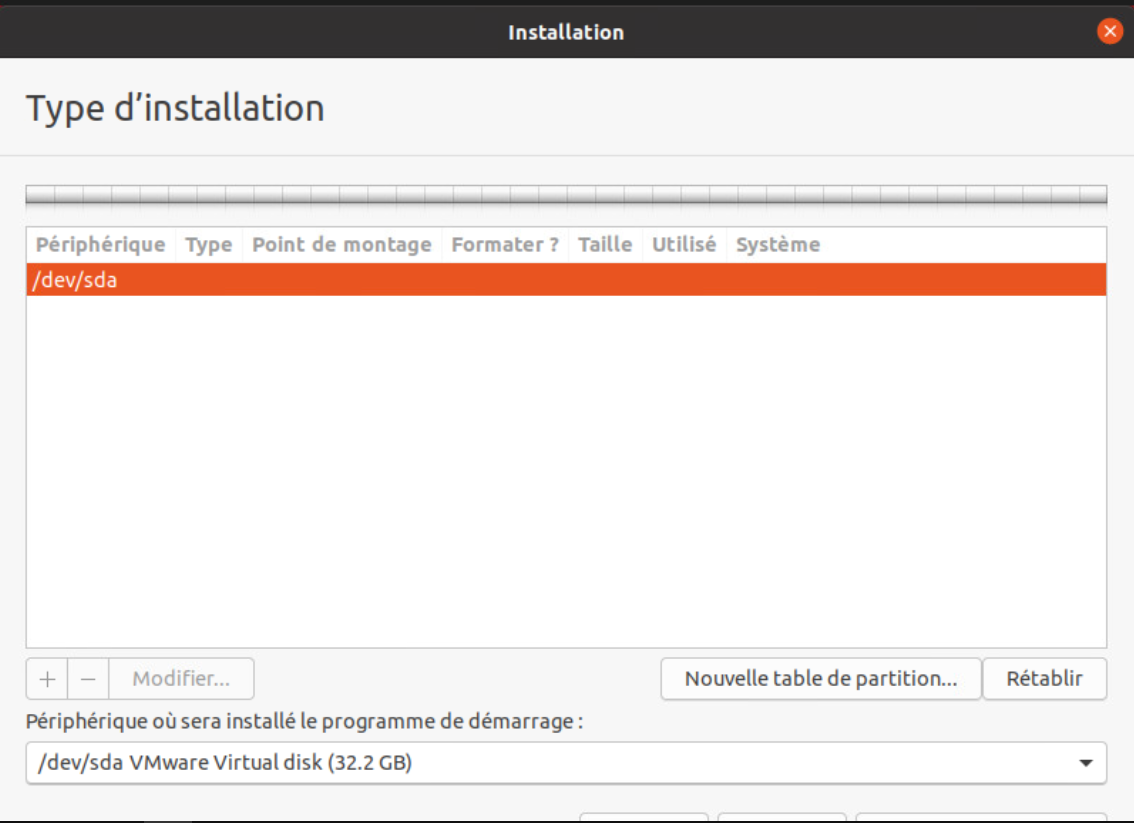
\includegraphics[scale=0.49]{images/Capture10}
		\end{figure}
		
		
		\item Nous aurons 4 partitions : 
		\begin{enumerate}[label=\arabic*)]
			\item Swap : mémoire virtuelle
			\item / (root) : espace du système d'exploitation
			\item /var : espace pour les fichiers variables. Logs, site web, bases de données, etc.
			\item /home : répertoires de données des utilisateurs.
		\end{enumerate}
		\item Suivez les prochaines étapes/images pour la création de ces partitions.
		\item Sélectionnez /dev/sda (Premier disque)
		\item Cliquez sur  {\color{blue}Nouvelle table de partition ...}
		\item Une fenêtre d'avertissement, figure~\ref{Fig9}, vous demande s'il faut créer une nouvelle table des partitions sur ce disque. Vous cliquez sur \textbf{Continuer} pour le faire.
		\begin{figure}[!htb]
			\centering
			\caption{\label{Fig9}Avertissement}
			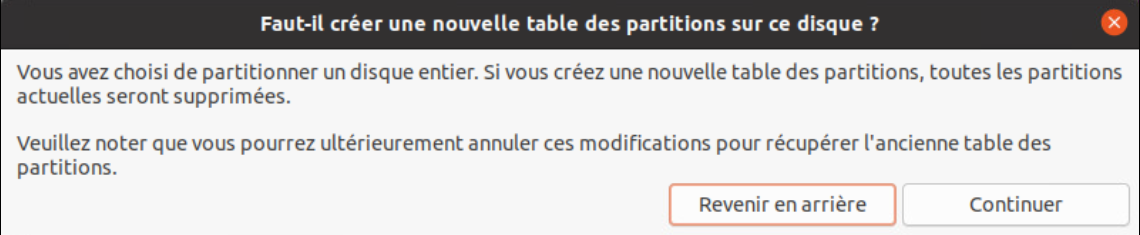
\includegraphics[scale=0.49]{images/Capture11}
		\end{figure}
		
		
		\item Sélectionnez espace libre et cliquez sur le  \textbf{+} pour créer une partition. Vous devriez avoir la figure~\ref{Fig10}
		
		\begin{figure}[!htb]
			\centering
			\caption{\label{Fig10}Créer une partition}
			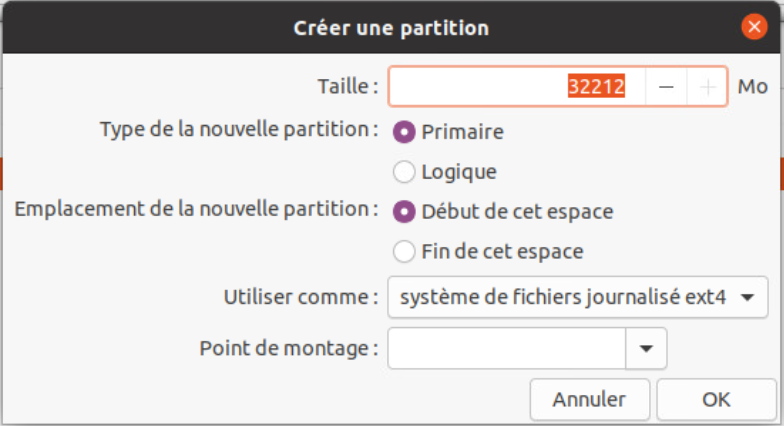
\includegraphics[scale=0.49]{images/Capture12}
		\end{figure}
		
		\item Modifier les valeurs pour correspondent à la figure~\ref{Fig11} créant ainsi la partition SWAP. Cliquez sur\textbf{ OK}.
		
		\begin{figure}[!htb]
			\centering
			\caption{\label{Fig11}Créer une partition SWAP}
			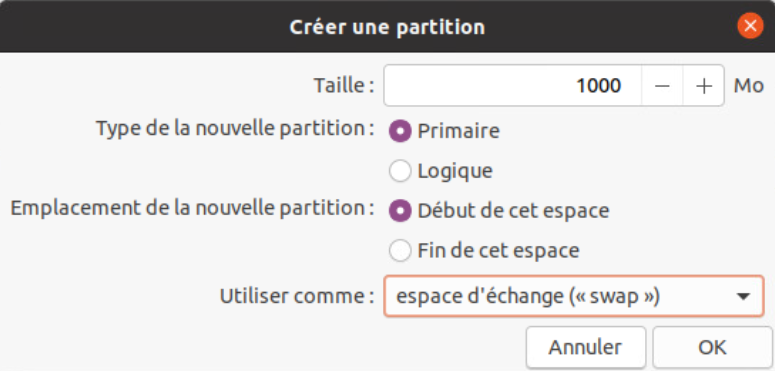
\includegraphics[scale=0.49]{images/Capture13}
		\end{figure}
		
		\item Sélectionnez espace libre et cliquez sur le  \textbf{+} pour créer une partition. 
		\item Modifier les valeurs pour correspondent à la figure~\ref{Fig12} créant ainsi la partition racine. {\color{blue}Faites très attention aux valeurs changées}: Taille, Type de la nouvelle partition, Système de fichier journalisé ext4, Point de montage. Cliquez sur\textbf{ OK}.
		
		\begin{figure}[!htb]
			\centering
			\caption{\label{Fig12}Créer une partition racine}
			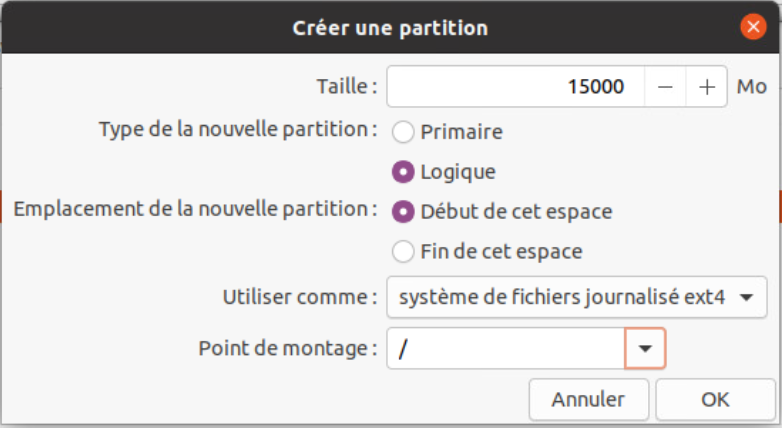
\includegraphics[scale=0.49]{images/Capture14}
		\end{figure}
		
		
		\item Voici ou vous en êtes après avoir cliqué sur OK : figure~\ref{Fig13}.
		
		\begin{figure}[!htb]
			\centering
			\caption{\label{Fig13}État du partitionnent}
			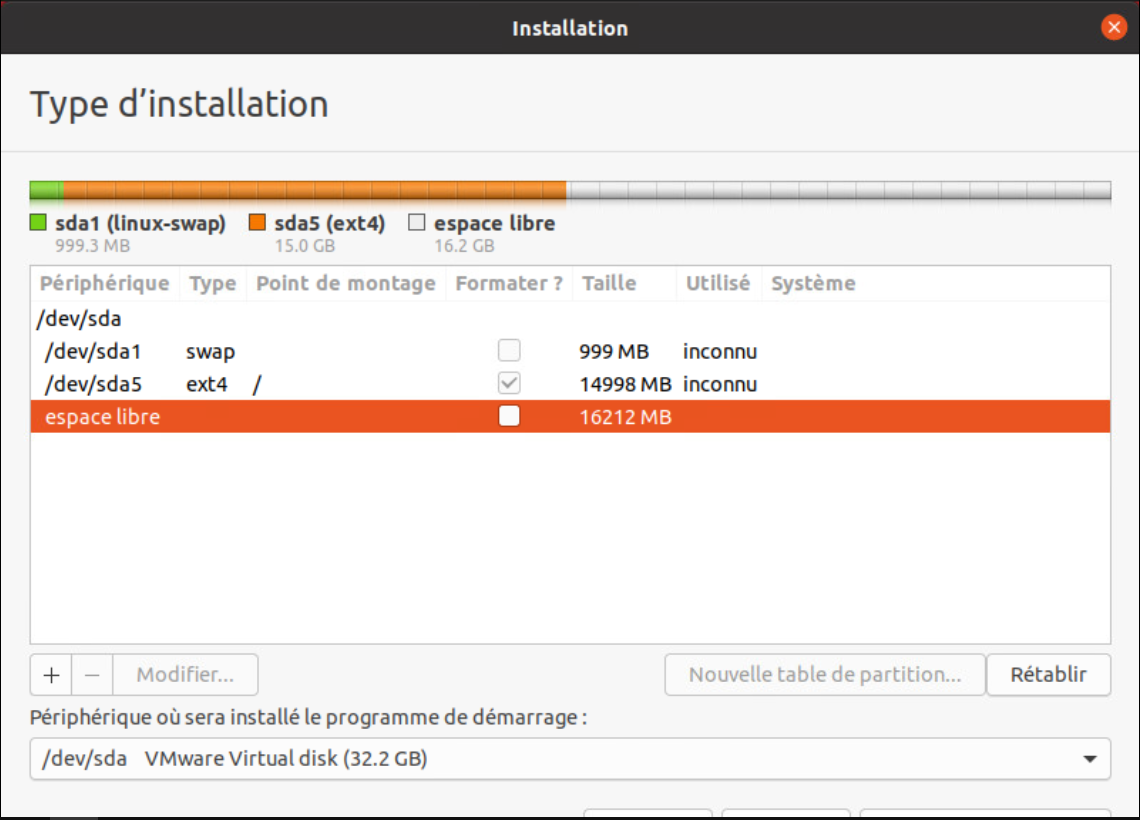
\includegraphics[scale=0.49]{images/Capture15}
		\end{figure}
		
		\item Sélectionnez espace libre et cliquez sur le  \textbf{+} pour créer une partition. 
		\item Modifier les valeurs pour correspondent à la figure~\ref{Fig14} créant ainsi la partition \\var. {\color{blue}Faites très attention aux valeurs changées}: Taille, Type de la nouvelle partition, Système de fichier journalisé ext4, Point de montage. Cliquez sur\textbf{ OK}.
		
		\begin{figure}[!htb]
			\centering
			\caption{\label{Fig14}Créer une partition avec var comme point de montage}
			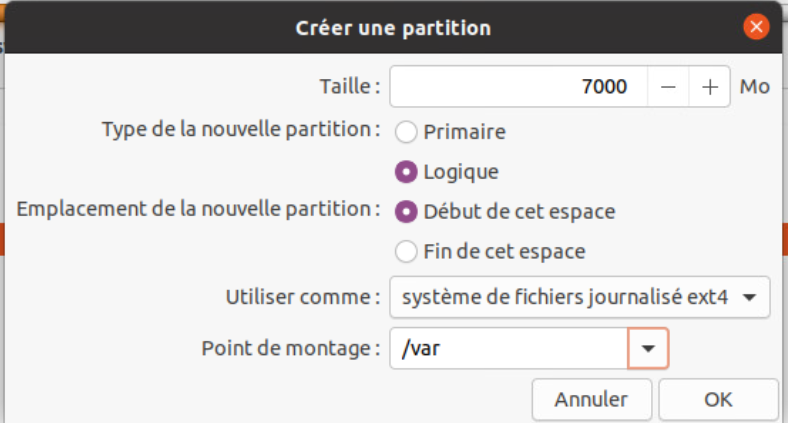
\includegraphics[scale=0.49]{images/Capture16}
		\end{figure}
		
		
		\item Sélectionnez espace libre et cliquez sur le  \textbf{+} pour créer une partition. 
		\item Modifier les valeurs pour correspondent à la figure~\ref{Fig15} créant ainsi la partition home. {\color{blue}Faites très attention aux valeurs changées}: Utilisez le reste du disque pour la taille, Type de la nouvelle partition, Système de fichier journalisé ext4, Point de montage. Cliquez sur\textbf{ OK}.
		
		
		\begin{figure}[!htb]
			\centering
			\caption{\label{Fig15}Créer une partition avec home comme point de montage}
			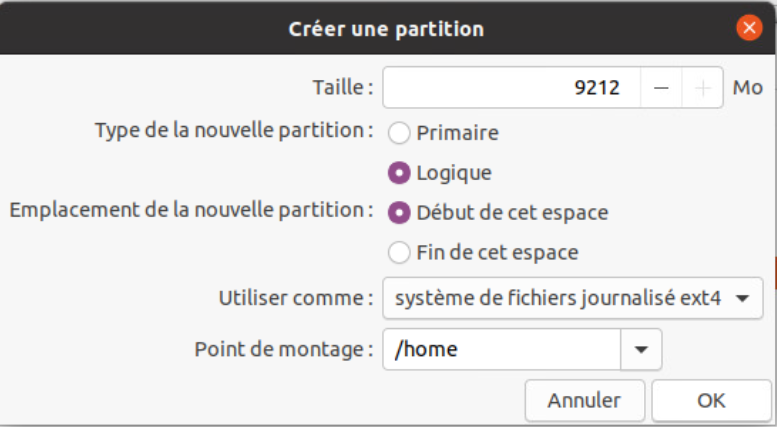
\includegraphics[scale=0.49]{images/Capture17}
		\end{figure}
		
		\item Vous avez maintenant un nouveau disque /dev/sda avec quatre (4) partitions comme à la figure~\ref{Fig16}.
		
		
		\begin{figure}[!htb]
			\centering
			\caption{\label{Fig16}État du disque /sda1}
			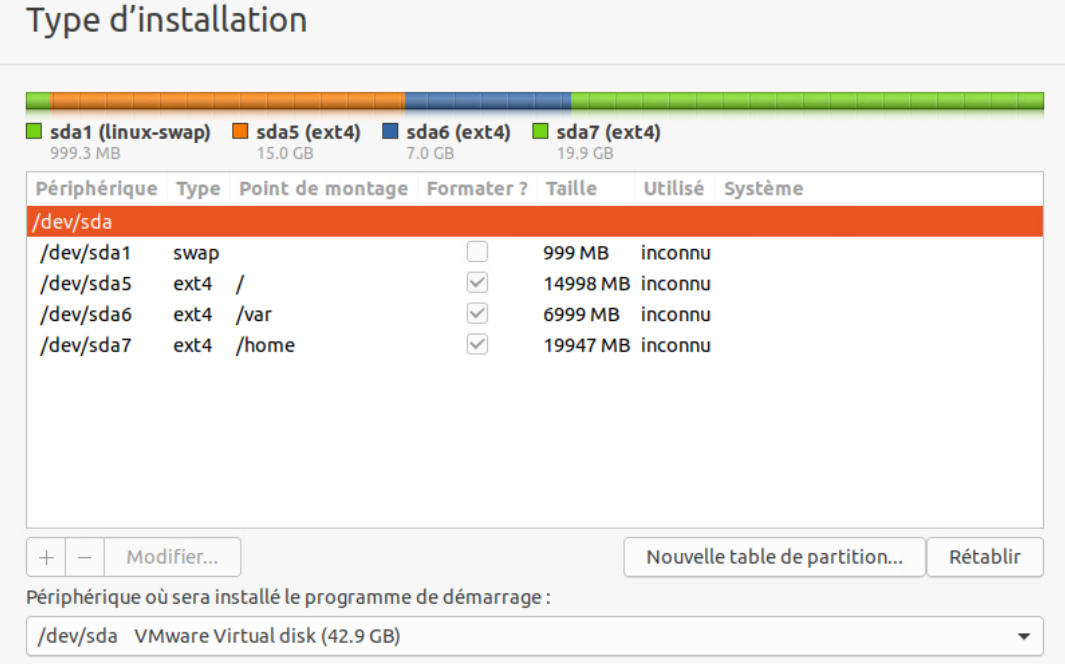
\includegraphics[scale=0.49]{images/Capture18}
		\end{figure}
		
		\fcolorbox{black}{orange}{ 
			\begin{minipage}{15cm}
				Attention : Dans mon cas, je ne voyais pas les boutons annuler et continuer. Il a donc fallu que j'utilise la touche tabulation pour me déplacer et déterminer lequel était le bon pour le bouton \textbf{Continuer}. Précédemment c'était toujours le dernier. Alors j'ai essayé le dernier et c'était le bon.
				
		\end{minipage}} 
		\vspace{10pt}  
		\begin{figure}[!htb]
			\centering
			\caption{\label{Fig16}État du disque /sda1}
			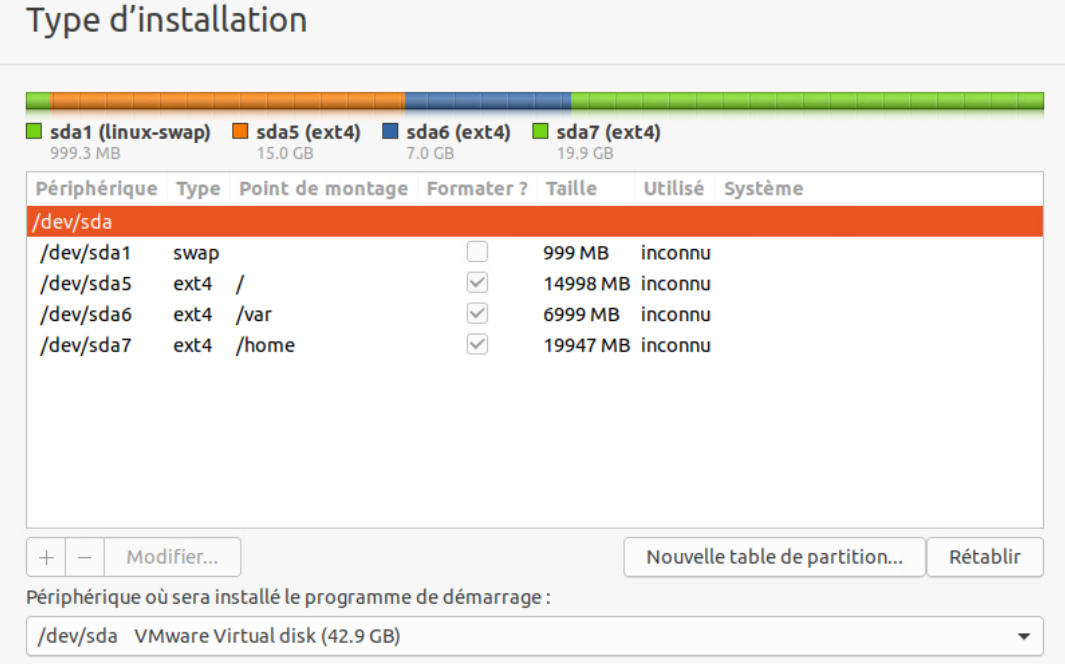
\includegraphics[scale=0.39]{images/Capture18}
		\end{figure}
		
		\item Une nouvelle fenêtre d'avertissement me demande s'il faut appliquer les changements sur les disques ? Vous répondez \textbf{Continuer} s'ils sont comme à la figure~\ref{Fig18}.
		
		\begin{figure}[!htb]
			\centering
			\caption{\label{Fig18}Avertissement}
			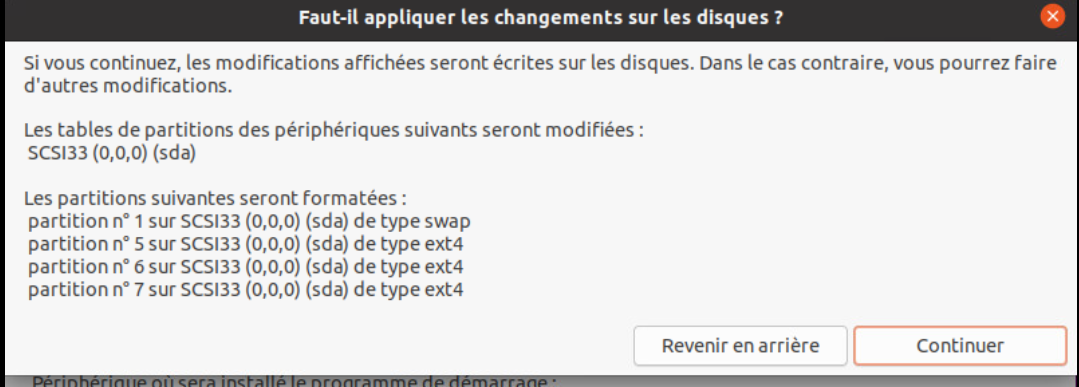
\includegraphics[scale=0.39]{images/Capture19}
		\end{figure}
		
		
		\item Indiquez le fuseau horaire (Toronto). Et cliquez sur \textbf{Continuer}.
		\item Qui êtes-vous ? Figure~\ref{Fig19}. Remplir les informations d'usager et mot de passe, donner un nom à votre ordinateur. Laisser la valeur par défaut : Demander mon mot de passe pour ouvrir une session. Cliquez sur \textbf{Continuer}.
		
		\begin{figure}[!htb]
			\centering
			\caption{\label{Fig19}Qui êtes-vous ?}
			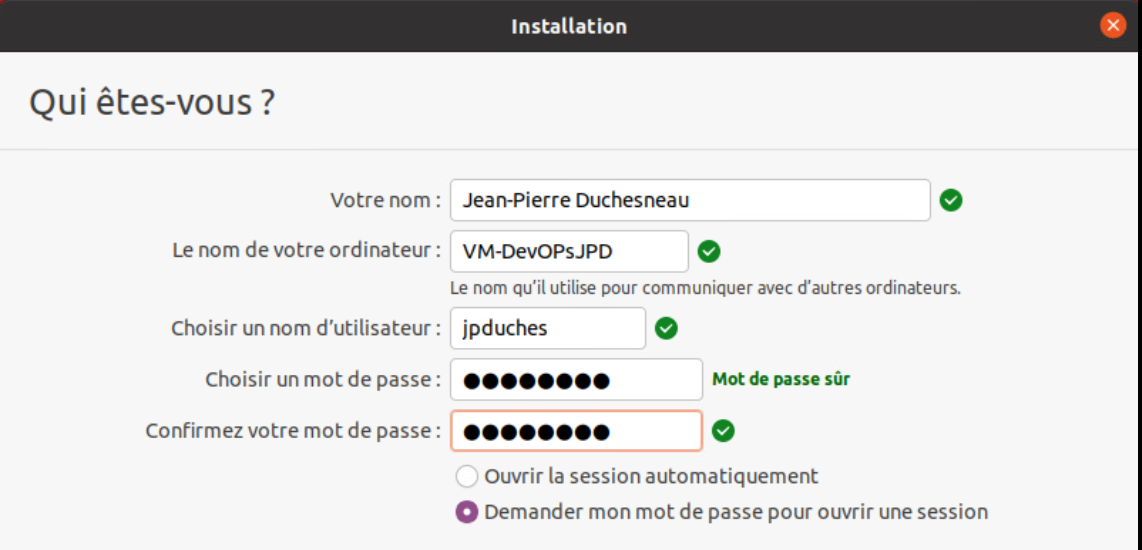
\includegraphics[scale=0.55]{images/Capture21}
		\end{figure} 
		
		\item La copie des fichiers est débutée. Relaxez-vous. {\color{orange}{\Huge \smiley{}}}
		
		\item Une dernière figure~\ref{Fig20} qui dit tout.
		\begin{figure}[!htb]
			\centering
			\caption{\label{Fig20}Installation terminée}
			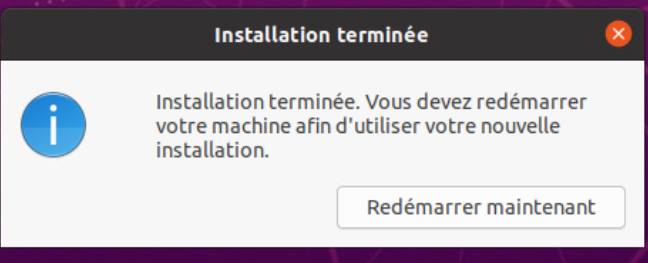
\includegraphics[scale=0.55]{images/Capture22}
		\end{figure} 
		
		\item Si ce n'est pas fait automatiquement, allez dans la configuration de votre VM et retiré le fichier ISO du lecteur CD/DVD en cliquant sur Déconnecter comme dans la figure~\ref{Fig21}.
		
		\begin{figure}[!htb]
			\centering
			\caption{\label{Fig21}Déconnecter le lecteur CD/DVD}
			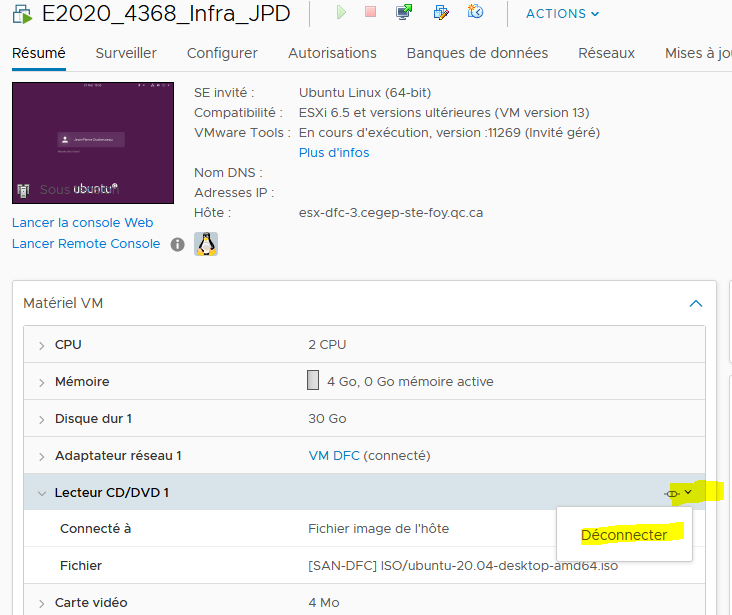
\includegraphics[scale=0.55]{images/Capture23}
		\end{figure}
		
		
	\end{itemize}
	
	\section{Première utilisation de votre machine} 
	
	
	
	Démarrez votre VM et connectez-vous.
	
	
	\subsection{Personnalisation du Bureau}
		\begin{itemize}
			\item Retirez toutes les icônes du lanceur qui sont inutiles. 
			\item Ajoutez l'icône terminal au lanceur.
			\item A titre d'exemple, voici ce que contient mon lanceur : 
			\begin{figure}[!htb]
				\centering
				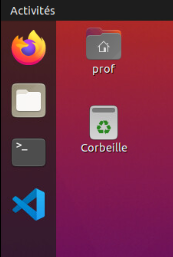
\includegraphics[scale=0.8]{images/lanceur}

			\end{figure}
		\end{itemize}
	\subsection{Vérification des partitions et du système}
	
	\subsubsection{Espace disque}
	\begin{itemize}
		\item  Ouvrez un terminal et taper les commandes demandées, attention ne tapez que ce qui suit le \$:
		
		
		\begin{lstlisting}[
		language=bash,
		]
		$df -h
		\end{lstlisting}
		\begin{figure}[!htb]
			\centering
			\includegraphics[scale=0.6]{images/captureDF}
			\caption{Espace disque après l'installation}
			\label{df}
		\end{figure}
		
		\item  \textbf{Question :} À quoi sert la commande {\color{blue}df} et son paramètre {\color{blue}-h} ?
		\item Utiliser la page {\color{blue}man} \footnote{man est une commande disponible sur les systèmes d'exploitation de type Unix. Elle permet de visionner les contenus d'une documentation formatée pour être exploitable par man et ce, en lien avec les commandes du SHELL. Vous pouvez trouver une version en français de ces pages à l'addresse : \url{http://manpagesfr.free.fr/}} pour répondre :
		\begin{lstlisting}[
		language=bash,
		]
		$man df
		\end{lstlisting}
		
		Cette commande vous permet d'avoir l'espace utilisé et disponible pour chaque partition du système de fichier qui est monté.\\
		Vous devriez pouvoir identifier vos partitions créées lors de l'installation.
		Le paramètre -h permet l'affichage à la puissance 1024 (exemple 1023M; 1024 donnant 1Go.).
		
		
		\item Essayer maintenant en lui passant la seconde commande grep. Nous affichons que ce qui concerne le disque dur sda : 
		\begin{lstlisting}[
		language=bash,
		]
		$df -h |grep 'sda'
		\end{lstlisting}
		
		\begin{figure}[!htb]
			\centering
			\includegraphics[scale=0.8]{images/captureDFGREP}
			\caption{Espace du disque SDA après l'installation}
			\label{dfGREP}
		\end{figure}
		
		Remarquez que j'ai mis un {\color{blue}H} plutôt qu'{\color{blue}h} miniscule. 
		
		\vspace{10pt}
		
		\textbf{Gestion des partitions, la commande fdisk :}
		\begin{itemize}
			\item  \textbf{fdisk} est un outil de base pour réaliser des opérations sur les tables de partitions des disques durs.  
			fdisk permet de manipuler les tables de partitions. Il permet de créer, de supprimer, de lister les partitions sur un disque dur. 
			
			\item taper la commande suivante, et avec la page man vérifer les informations données sur la commande.
			\begin{lstlisting}[language=bash]   ]
			$sudo fdisk -l /dev/sda
			\end{lstlisting} 
		\end{itemize}
		
		\begin{figure}[!htb]
			\centering
			\includegraphics[scale=0.8]{images/captureFDISK}
			\caption{Gestion du disque SDA avec la commande FDISK}
			\label{fdisk}
		\end{figure}
		\item Il  est également possible d'avoir des informations en mode graphique. Pour ce faire, utiliser l'outil disk. Vous devriez avoir l'image suivante :
		\begin{figure}[!htb]
			\centering
			\includegraphics[scale=0.5]{images/captureB1}
			\caption{Espace du disque SDA avec l'utilitaire graphique}
			\label{Disk}
		\end{figure}
		\item Cliquez sur chaque partition pour pouvoir accéder aux informations. Vérifier les points de montage.
		\item Finalement, pour voir les partitions qui seront monté au démarrage, affiché le fichier /etc/fstab :
		\begin{lstlisting}[language=bash]   ]
		$ cat /etc/fstab
		\end{lstlisting} 
		\item Pour bien comprendre le rôle du fichier fstab, voup pouvez lire la page man fstab ou encore allez lire la documentation suivante : \url{https://doc.ubuntu-fr.org/mount_fstab}
	\end{itemize}
	
	\subsubsection{Mémoire RAM, processeur et processus }
	
	\begin{itemize}
		\item  Dans un terminal, taper la commande {\color{blue}top}
		
		\begin{lstlisting}[language=bash]   ]
		$top
		\end{lstlisting}
		La commande top vous permet d'avoir une vue dynamique en temps réel du processus, de la mémoire et du processeur.
		
		\begin{figure}[!htb]
			\centering
			\includegraphics[scale=0.65]{images/captureTOP}
			\caption{Commande top}
			\label{top}
		\end{figure}
		\item Pour quittez top taper {\color{blue}q}.
	\end{itemize}
	
	\subsection{Création de clés SSH}
	
	
	\textbf{SSH} est un protocole permettant d'établir une communication chiffrée, donc sécurisée (on parle parfois de tunnel), sur un réseau informatique (intranet ou Internet) entre une machine locale (le client) et une machine distante (le serveur). Vous aurez à l'utiliser régulièrement soit pour gérer une machine distante ou encore pour vous connecter avec GIT sur un dépôt distant.\\
	
	\textbf{OpenSSH} est la solution la plus utilisée pour mettre en place une communication SSH via un ensemble d'outils libres dont certains sont installés par défaut sur Ubuntu.
	
	\textbf{Nous allons créer votre clé privée et publique :}
	
	\begin{itemize}
		\item Ouvrez un terminal.
		
		\item Générez une nouvelle paire de clés SSH ED25519 avec votre adresse courriel du Cégep :
		
		\begin{lstlisting}[language=bash]   ]
		$ssh-keygen -t ed25519 -C "email@example.com"
		\end{lstlisting}
		L'option -C ajoute un commentaire, ici l'adresse, dans la clé au cas où vous en auriez plusieurs et je veux savoir de quelle clé il s'agit. C'est facultatif.
		
		\item Ensuite, vous serez invité à entrer un chemin de fichier pour enregistrer votre paire de clés SSH. Utilisez le chemin suggéré en appuyant sur
		{\color{blue}entrer}. L'utilisation du chemin suggéré permettra normalement à votre client SSH
		d'utiliser automatiquement la paire de clés SSH sans configuration supplémentaire.
		Cette paire de clés SSH sera utilisée dans votre dossier 
		\verb! ~/.ssh /!
		\item à la question\textbf{ Enter passphrase} (empty for no passphrase): laisser vide et taper {\color{blue}enter}.
		\item Si tous a bien fonctionné, vous devriez  avoir des informations qui ressemblent à ceci : 
		\begin{figure}[!h]
			\centering
			\includegraphics[scale=0.6]{images/captureb2}
		\end{figure}
		\item Vous pouvez vérifier la présence de votre paire de clés en tapant :
		\begin{lstlisting}[language=bash]   ]
		$cd .ssh
		$ls -l
		\end{lstlisting}
		\item {\color{red}Attention :} La clé sans extension ne doit pas être partagée. C'est la clé privée.
		\item Vous pourrez, la cas échéant, partager votre clé publique (celle ayant l'extension .pub) sur des serveurs pour automatiser votre connexion sécurisée avec SSH.
	\end{itemize}
	
	
	\vspace{2cm}
	\textbf{ Fin de l'exercice \exercice.}
	
	
	
	
	
	
	
	\section{Compétences développées en partie dans l'exercice \exercice}
	\begin{tabular}{|p{5cm}|l|}
		\hline
		\textbf{Énoncé(s) de compétence}&\textbf{Élément de la compétence} \\[3pt]
		\hline
		00Q1 - Effectuer l’installation et la gestion d’ordinateur&2 installer le système d’exploitation.\\
		&3 Installer des applications\\
		&4 Effectuer des tâches de gestion du système d’exploitation.\\
		\hline
		00SF - Évaluer des composants logiciels et
		matériels&1 Rechercher des composants logiciels et matériels.\\
		&2 Formuler des avis sur les composants logiciels et matériels.\\
		\hline
		
	\end{tabular}
	
	
	
	
	\pagebreak
	
	\renewcommand{\contentsname}{Sommaire} % Dans le corps du document,avant la commande \tableofcontents.
	
	\setcounter{tocdepth}{5}
	
	\addcontentsline{toc}{section}{Sommaire}
	
	\tableofcontents
	
	\pagebreak
	
	
	\addcontentsline{toc}{section}{Références}
	
	\nocite{*}
	
	
	
	% \textbf{Cette liste de références contient également des lectures suggérées pour approfondir le sujet.}\\
	
	\printbibliography
	
	
	% \rule{\linewidth}{1pt}\\
	
	\textbf{\textit{Ce document a été écrit avec LaTeX}.}\\
	
	%\includegraphics[scale=1]{88x31.png}\\
	
	\shadowbox{\parbox{15cm}
		{Cette oeuvre, création, site ou texte est sous licence Creative Commons Attribution - Pas d’Utilisation commerciale - Partage dans les Mêmes Conditions 4.0 International. Pour accéder à une copie de cette licence, merci de vous rendre à l'adresse suivante \url{http://creativecommons.org/licenses/by-nc-sa/4.0/} \\ ou envoyez un courrier à Creative Commons, 444 Castro Street, Suite 900, Mountain View, California, 94041, USA.}}
	
\end{document}

